\documentclass[12pt]{article}
\usepackage{graphicx}
\graphicspath{ {../Data/} }

\title{Temporal autocorrelation of the temperature in Key West, Florida during the 20th century}

\author{Ioan Evans}

\date{07/11/2020}

\begin{document}
    \maketitle

    \begin{abstract}
        Temperature displays an autocorrelation effect, whereby sucessive years have more similar temperatures than more 
        distant years. 
    \end{abstract}

    \begin{figure}[h!]
        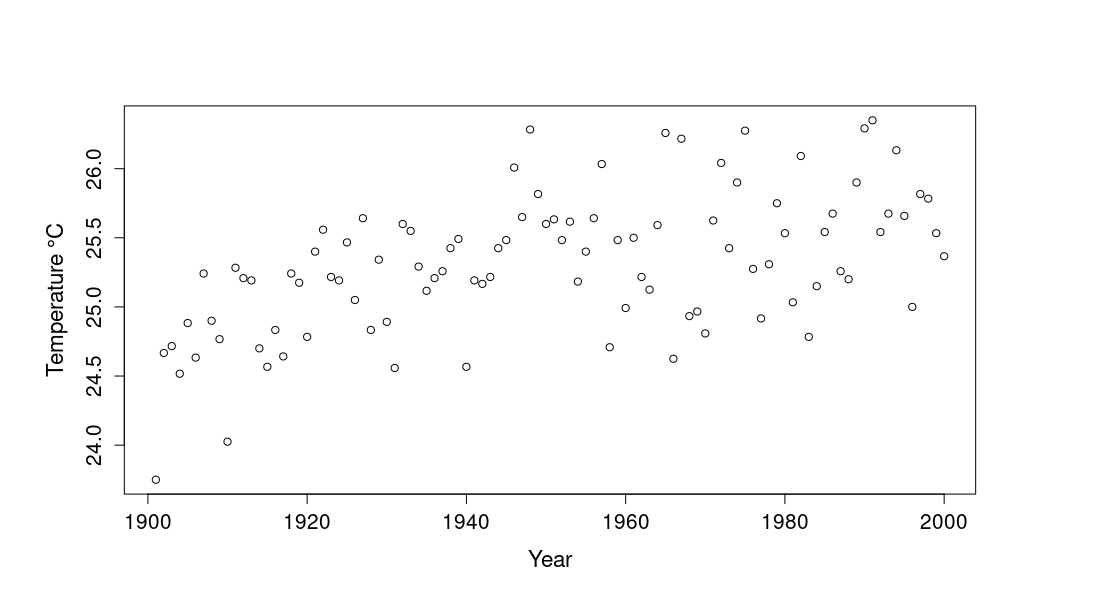
\includegraphics[width=15cm]{Fig3}
        \centering
        \caption{Teperature in Key West, Flordia during the 20th century.}
    \end{figure}

    \section{Materials \& Methods}
        Temperature data is from Key West, Florida and collected between 1901 and 2000 (Fig. 1).
        
        Autocorrelation is computed by calculating the correlation between successive years (t and t-1).
        A significance value (p-value) is obtained by comparing the correlation of the temperature data ordered by year, to 
        correlation between temperature data that has been randomly permutated (n = 10,000; Fig. 2)). Correlation 
        coefficients of the permuted data are calculated by comparing successive values. The significance value is taken 
        as the number of times the correlation of permuted data is greater than the correlation of ordered data, divided 
        by the number of iterations (10,000).

    \begin{figure}[h!]
        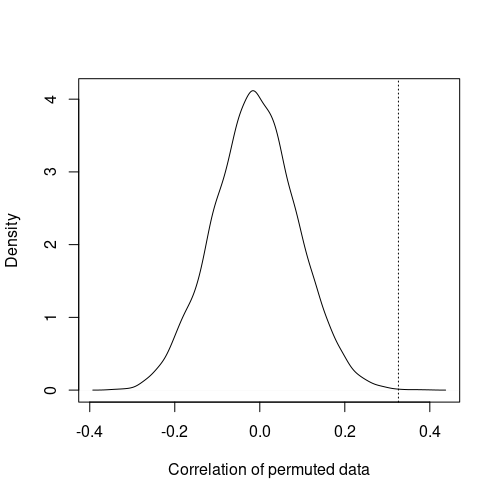
\includegraphics[width=10cm]{Fig2}
        \centering
        \caption{Density plot of the correlations between successive values of randomly permuted temperature data (n = 10,000).
         The dotted line indicates the correlation between successive years of the ordered temperature data (0.326).}
    \end{figure}

    \section{Results}
        The correlation between successive years (0.326) returns a p-value of less than 0.001 (Fig.2). The 
        observed correlation occurs in fewer than 10 in 10,000 iterations of the randomly permuted data. 

    \section{Discussion}
        The results suggest that temperature displays a significant autocorrelative effect between successive years. The 
        relationship between successive years displays a moderate correlation. Therefore, the temperature of any year is 
        predicted to have a significant effect on the temperature of the following year, however, other factors will 
        contribute to the observed variation in the data.

\end{document}